\chapter{Chapitre 3 : Conception et Modélisation}
\thispagestyle{fancy}
\newpage

\section{Introduction}
La première phase du projet a été consacrée à la conception initiale, à la définition de l'architecture backend et des bases de données, ainsi qu'à la création des premiers diagrammes UML.

\section{Méthodologie Adoptée}
La méthodologie adoptée pour la conception du système s'est basée sur une approche structurée et itérative.

\subsection{Modèle en cascade}
Pour la phase de conception, nous avons adopté une approche en cascade adaptée, permettant de définir clairement les étapes successives tout en maintenant la possibilité de réviser les décisions précédentes au besoin.

\subsection{Langage UML}
Le langage UML (Unified Modeling Language) a été utilisé comme standard pour représenter graphiquement l'architecture et les interactions du système. Ce choix permet une communication claire et non ambiguë entre toutes les parties prenantes du projet.

\section{Conception}

\subsection{Identification des acteurs}
Les principaux types d'utilisateurs identifiés pour la plateforme sont :
\begin{itemize}
  \item \textbf{Apprenant Individuel :} S'inscrit, s'abonne, apprend, demande des consultations
  \item \textbf{Employé d'Entreprise :} Apprend via l'abonnement de l'entreprise, demande des consultations
  \item \textbf{Administrateur/Manager d'Entreprise :} Gère le compte de l'entreprise, les employés, les abonnements, attribue les cours, consulte les analyses
  \item \textbf{Créateur de Cours :} Conçoit et élabore le contenu des cours (modules, leçons, quiz)
  \item \textbf{Consultant/Fournisseur de Prestations :} Gère sa disponibilité, anime les sessions via la plateforme de réunion
  \item \textbf{Agent de Support Plateforme :} Assiste les utilisateurs pour les problèmes liés à la plateforme et les questions-réponses
  \item \textbf{Administrateur de la Plateforme :} Supervise l'ensemble de la plateforme, les utilisateurs, le contenu, les paramètres
\end{itemize}

\subsection{Identification des messages}
La plateforme e-learning conçue repose sur les fonctionnalités essentielles suivantes :
\begin{itemize}
    \item \textbf{E-Learning :}
    \begin{itemize}
        \item Catalogue de cours (filtrable, consultable)
        \item Modules, Leçons (vidéo, basées sur des images)
        \item Quiz et Évaluations
        \item Suivi de la Progression
        \item Certificats de Réussite
        \item Support Multilingue (EN/FR)
        \item Paramètres Utilisateur et Entreprise
    \end{itemize}
    \item \textbf{Consultation et Prestation :}
    \begin{itemize}
        \item Navigation des services
        \item Profils des consultants et disponibilité
        \item Système de réservation/demande
        \item Intégration API avec la plateforme de réunion personnalisée
        \item Facturation des sessions
    \end{itemize}
    \item \textbf{Monétisation :}
    \begin{itemize}
        \item Abonnements pour utilisateurs individuels (accès illimité)
        \item Abonnements pour entreprises (par utilisateur)
        \item Réductions et Démos
    \end{itemize}
\end{itemize}

\subsection{Les diagrammes de cas d'utilisation}
Les diagrammes de cas d'utilisation ont permis de représenter visuellement les interactions entre les acteurs et le système.

\begin{figure}[h!]
  \centering
  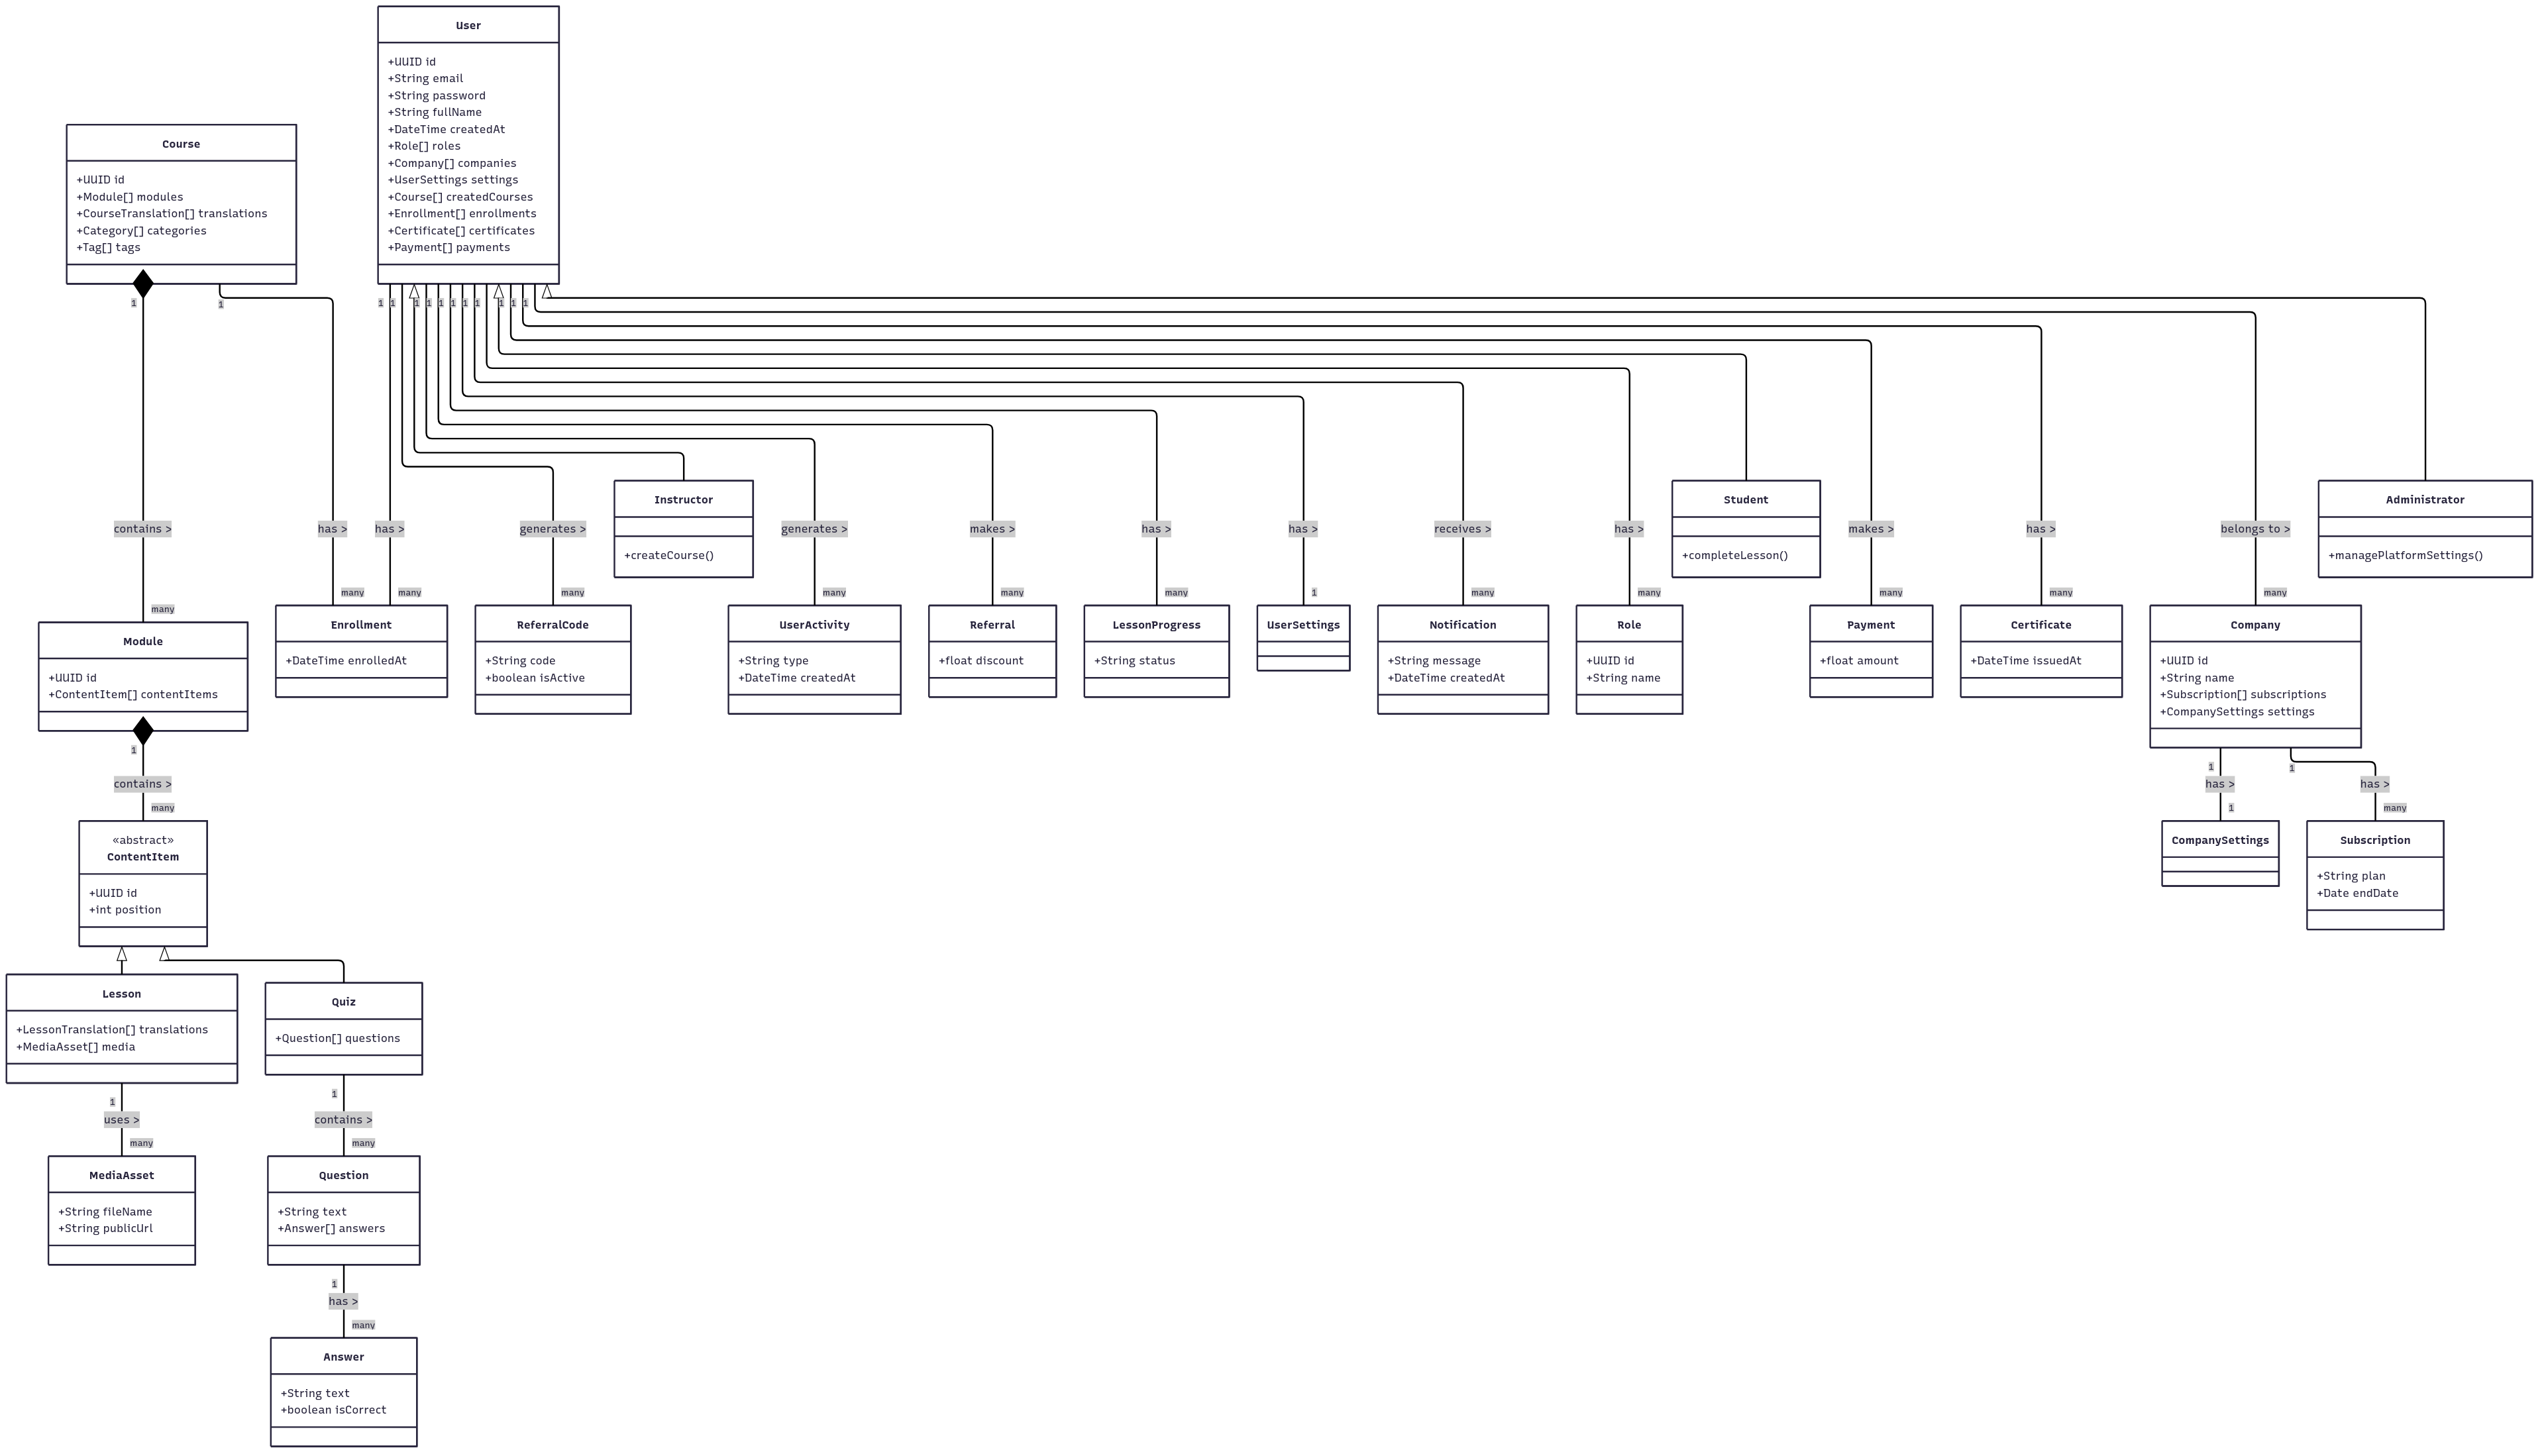
\includegraphics[width=0.9\textwidth,keepaspectratio]{class_diagrame.png}
  \caption{\textbf{Diagramme de cas d'utilisation} montrant les principales fonctionnalités accessibles par les acteurs.}
  \label{fig:usecase_diagram}
\end{figure}

\subsection{Les diagrammes de séquence}
Les diagrammes de séquence ont permis d'illustrer les interactions temporelles entre les différents composants du système pour des scénarios clés.

Pour illustrer le fonctionnement de l'architecture, voici un exemple de flux de communication entre les services pour un scénario d'inscription et d'abonnement :
\begin{enumerate}
  \item \textbf{Client (Next.js)} $\rightarrow$ \textbf{Passerelle API (Nginx)} $\rightarrow$ \textbf{Service IAM} (Création de l'utilisateur)
  \item \textbf{Service IAM} $\rightarrow$ \textbf{Kafka} (Publie `UserRegisteredEvent`)
  \item \textbf{Service de Notification} (Consomme l'événement) $\rightarrow$ Envoie un Email de Bienvenue
  \item \textbf{Client} $\rightarrow$ \textbf{Passerelle API} $\rightarrow$ \textbf{Service de Facturation} (Demande d'abonnement)
  \item \textbf{Service de Facturation} $\rightarrow$ Passerelle de Paiement et Mise à jour de la BD interne
  \item \textbf{Service de Facturation} $\rightarrow$ \textbf{Kafka} (Publie `SubscriptionActivatedEvent`)
  \item \textbf{Service IAM} (Consomme, met à jour le statut utilisateur) \& \textbf{Service de Notification} (Consomme, envoie une confirmation)
\end{enumerate}

\begin{figure}[h!]
  \centering
  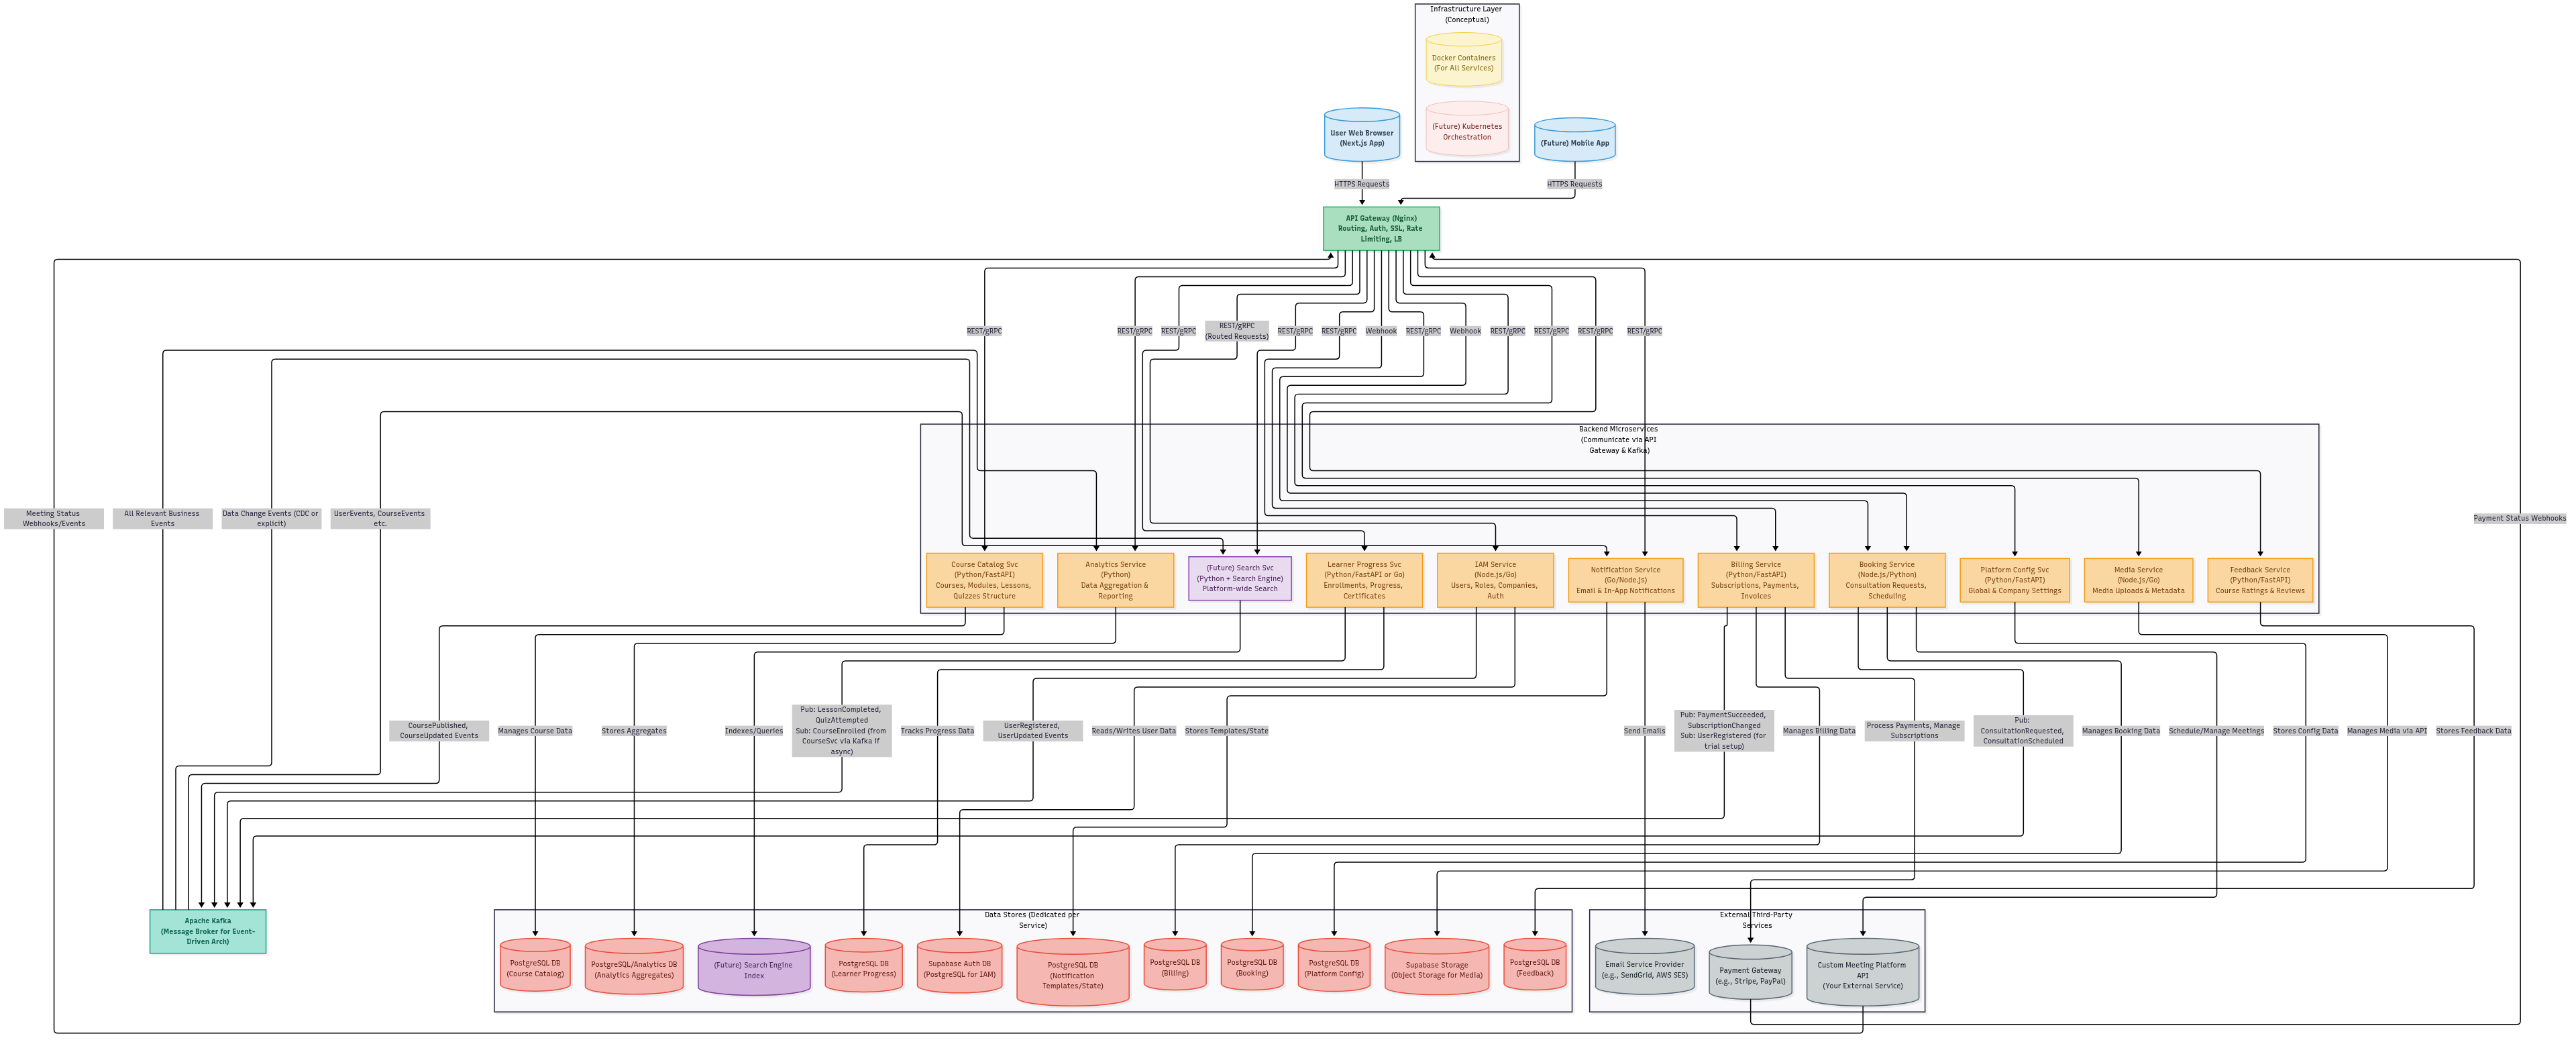
\includegraphics[width=0.9\textwidth,keepaspectratio]{archetecture_diagrame.png}
  \caption{\textbf{Diagramme de séquence} illustrant le processus d'inscription et d'abonnement.}
  \label{fig:sequence_diagram}
\end{figure}

\subsection{Le diagramme de classes}
Le diagramme de classes a été élaboré pour représenter les principales entités du système et leurs relations.

\begin{figure}[h!]
  \centering
  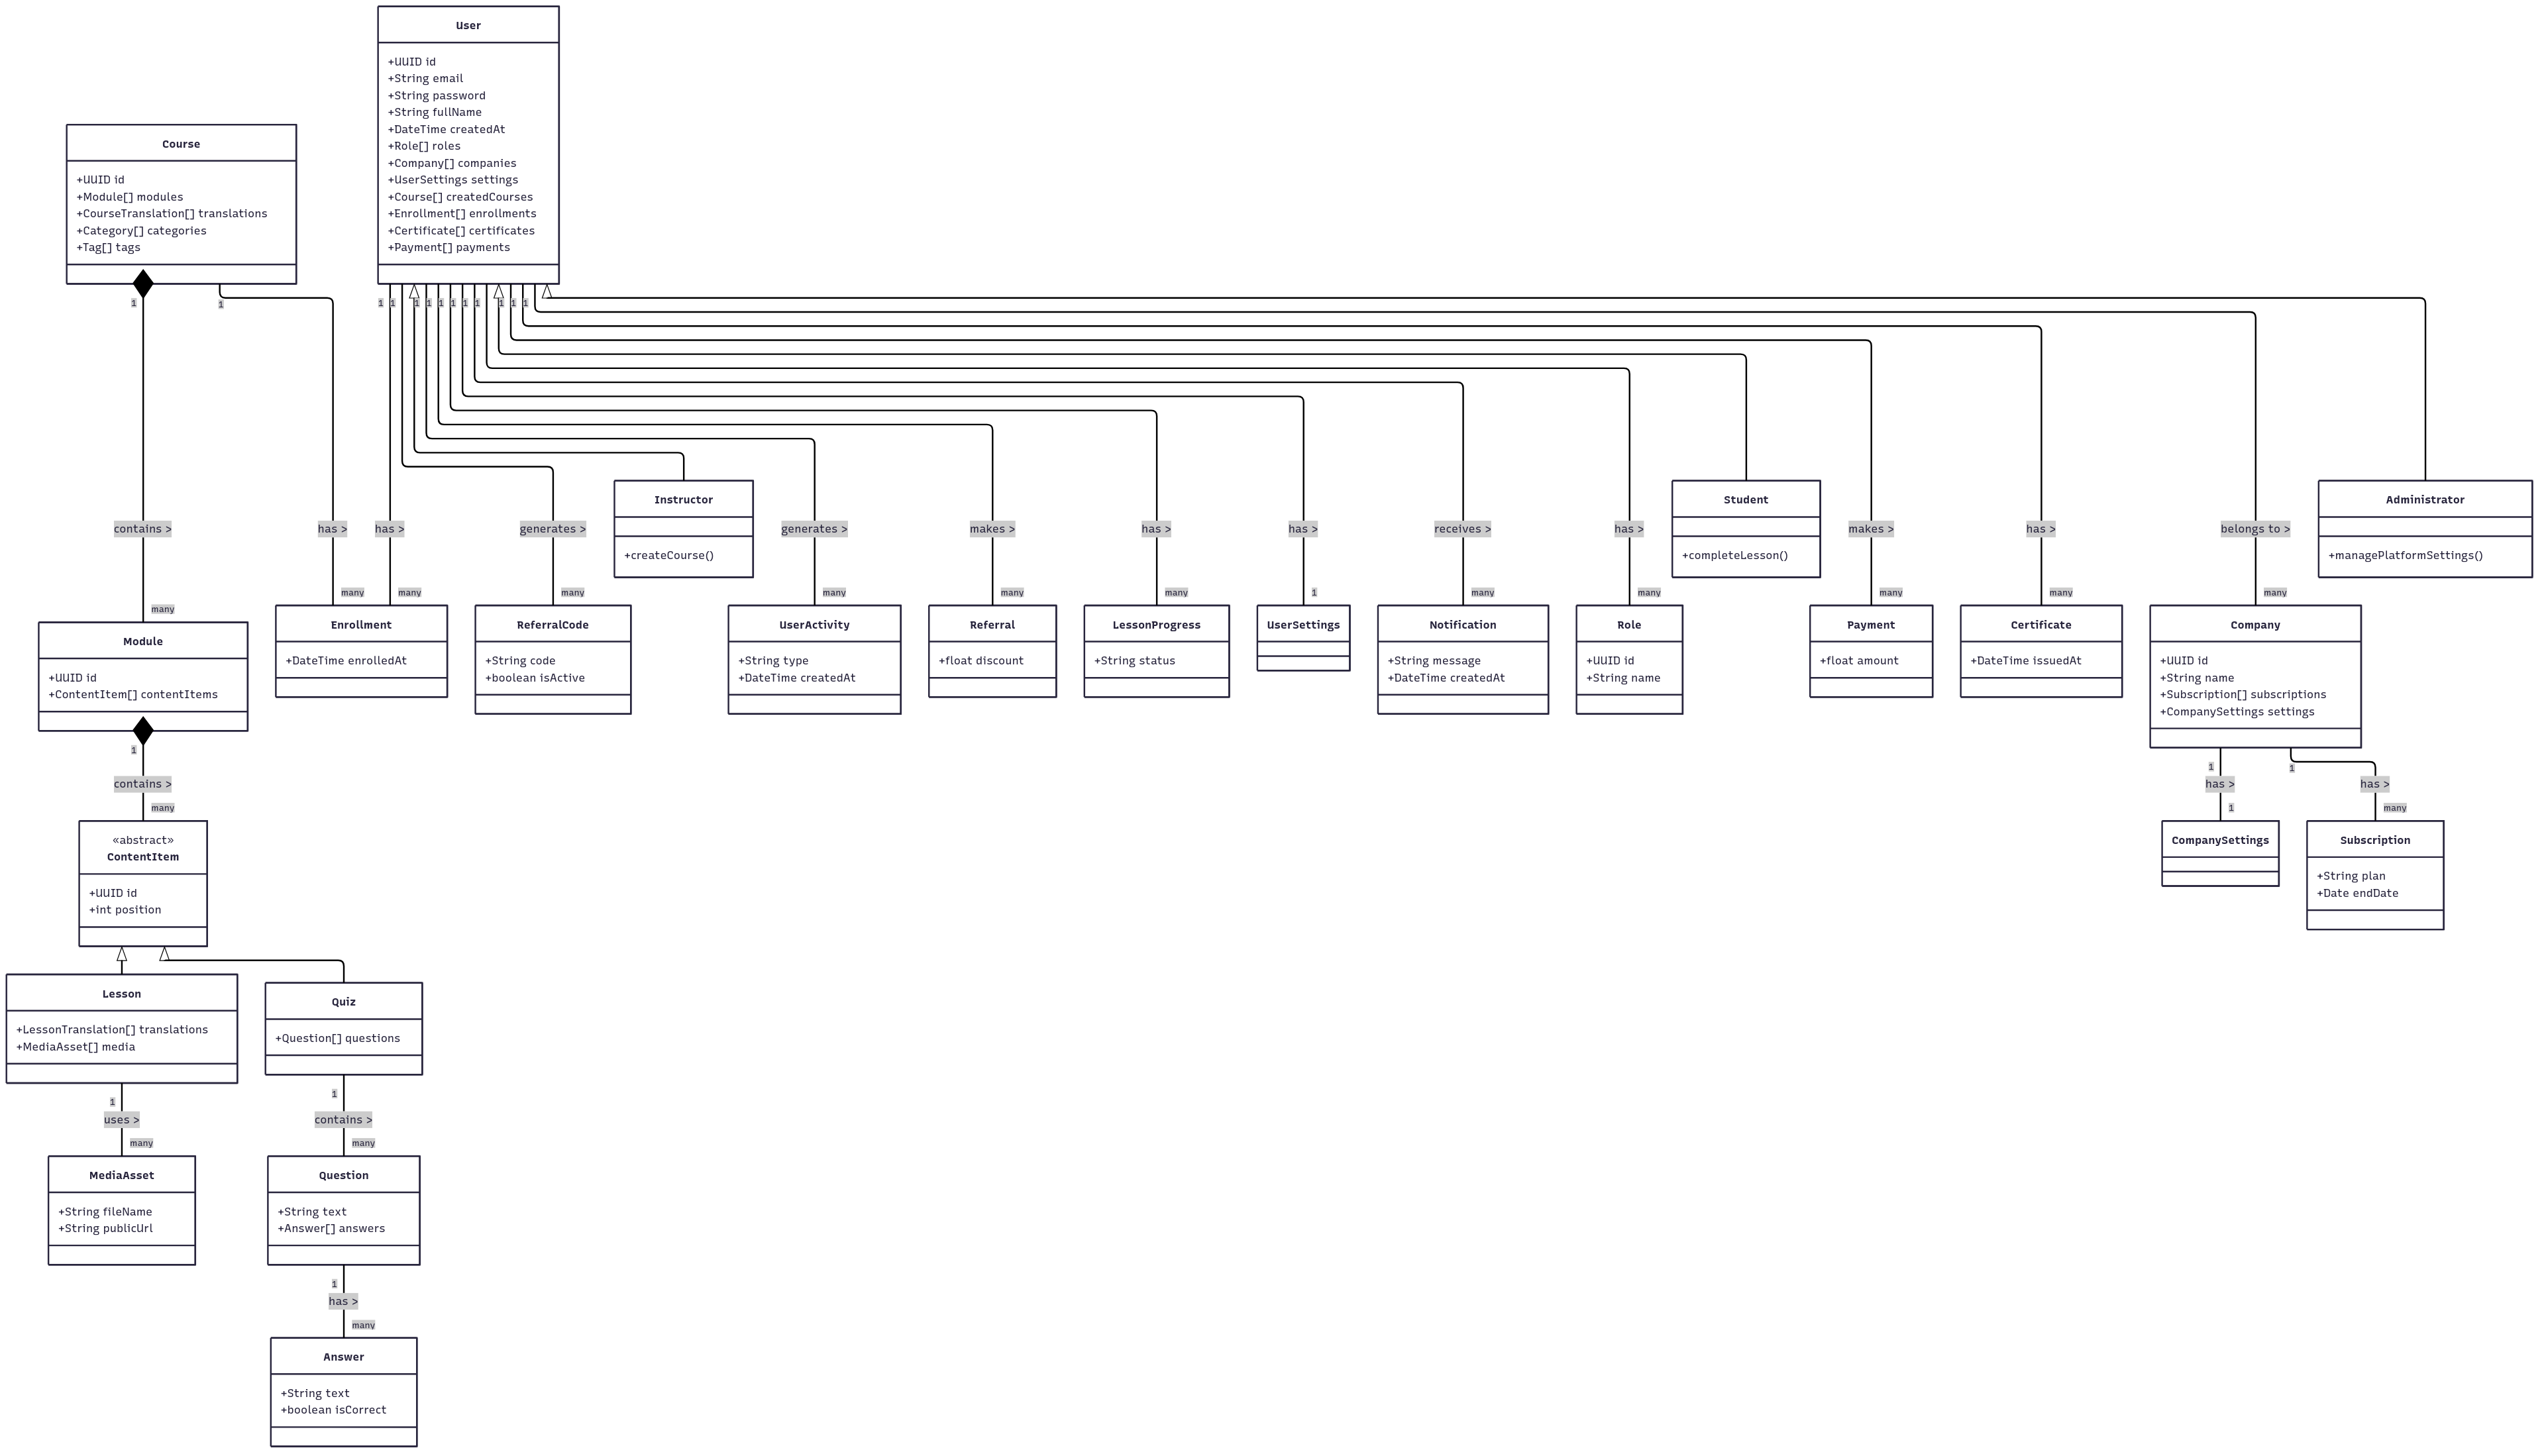
\includegraphics[width=0.9\textwidth,keepaspectratio]{class_diagrame.png}
  \caption{\textbf{Diagramme de classes} de la plateforme e-learning montrant les principales entités et leurs relations.}
  \label{fig:class_diagram}
\end{figure}

Ce diagramme illustre les relations entre les différentes entités du système, comme les utilisateurs, les cours, les modules, les leçons, les abonnements et les services de consultation. Les cardinalités et les types de relations (composition, agrégation, héritage) ont été définies pour refléter précisément la structure du modèle de données.

\section{Architecture Adoptée}

L'architecture envisagée pour la plateforme repose sur une approche de microservices, justifiée par plusieurs avantages clés :
\begin{itemize}
  \item \textbf{Scalabilité :} Mise à l'échelle indépendante des services individuels selon les besoins
  \item \textbf{Maintenabilité :} Possibilité de modifier des parties spécifiques sans impacter l'ensemble du système
  \item \textbf{Résilience :} Limitation de l'impact des défaillances à des services spécifiques
  \item \textbf{Autonomie des Équipes :} Développement, tests et déploiement indépendants par différentes équipes
  \item \textbf{Flexibilité Technologique :} Utilisation des technologies les plus adaptées pour chaque service
\end{itemize}

\subsection{Pile Technologique}
La pile technologique définie pour le développement comprend :
\begin{itemize}
  \item \textbf{Frontend :} Next.js (React)
  \item \textbf{Microservices Backend :}
    \begin{itemize}
      \item Go (pour les services critiques en performance et concurrents comme les Notifications, le backend de la plateforme de réunion)
      \item Python avec FastAPI (pour les services gourmands en données, développement rapide d'API, par exemple, Catalogue de Cours, Facturation)
      \item Node.js avec Express (TypeScript) (pour les opérations I/O intensives, interaction Supabase, par exemple, IAM, Gestion des Médias)
    \end{itemize}
  \item \textbf{Bases de Données :}
    \begin{itemize}
      \item PostgreSQL (stockage relationnel principal pour la plupart des services)
      \item Supabase (pour l'Authentification, le Stockage, et son Postgres géré pour des services spécifiques)
    \end{itemize}
  \item \textbf{Passerelle API :} Nginx (en tant que reverse proxy et passerelle)
  \item \textbf{Broker de Messages :} Apache Kafka (pour une gestion d'événements asynchrones robuste et scalable)
  \item \textbf{Conteneurisation et Orchestration :} Docker (Kubernetes serait une étape logique suivante pour l'orchestration)
\end{itemize}

\subsection{Modèles de Données des Services}
Dans le cadre de cette première phase, des modèles de données préliminaires ont été conçus pour chacun des services identifiés. Voici quelques exemples des structures de données principales :

\newpage
\subsubsection{Service IAM (Identity and Access Management)}
\begin{figure}[h!]
  \centering
  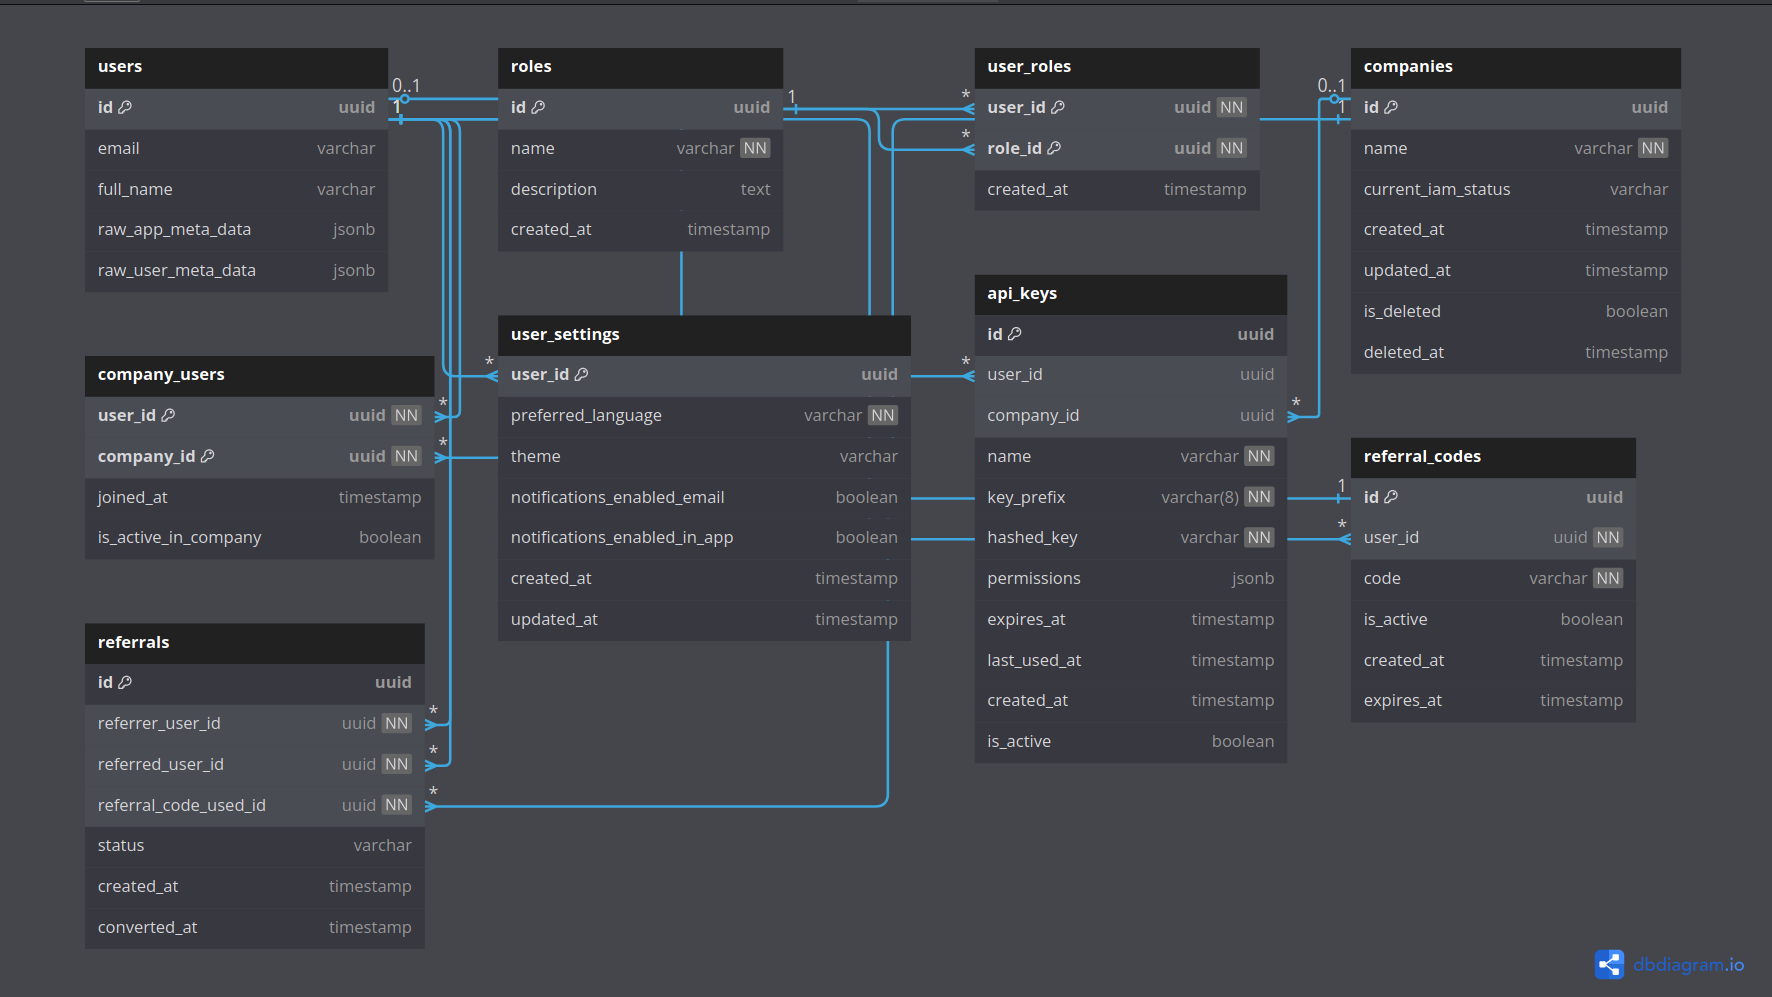
\includegraphics[width=0.8\textwidth,keepaspectratio]{services_db_screanshots/Screenshot 2025-06-06 at 15-08-36 IAM_Service.pdf.png}
  \caption{\textbf{Modèle de données du service IAM} pour la gestion des utilisateurs et des accès.}
  \label{fig:iam_service}
\end{figure}
\vspace{-10pt}
\small
\paragraph{Points clés du modèle IAM :}
\begin{itemize}[leftmargin=*,noitemsep,topsep=0pt]
  \item \textbf{Gestion centralisée des utilisateurs} avec tables dédiées aux utilisateurs, rôles et permissions
  \item \textbf{Support multi-tenant} via la table des entreprises (companies)
  \item \textbf{Système de référence} permettant le suivi des recommandations et affiliations
  \item \textbf{Paramètres utilisateurs} stockés de manière structurée pour personnaliser l'expérience
  \item \textbf{Jetons d'authentification} permettant une gestion sécurisée des sessions
\end{itemize}
\normalsize
\newpage

\subsubsection{Service de Contenu}
\begin{figure}[h!]
  \centering
  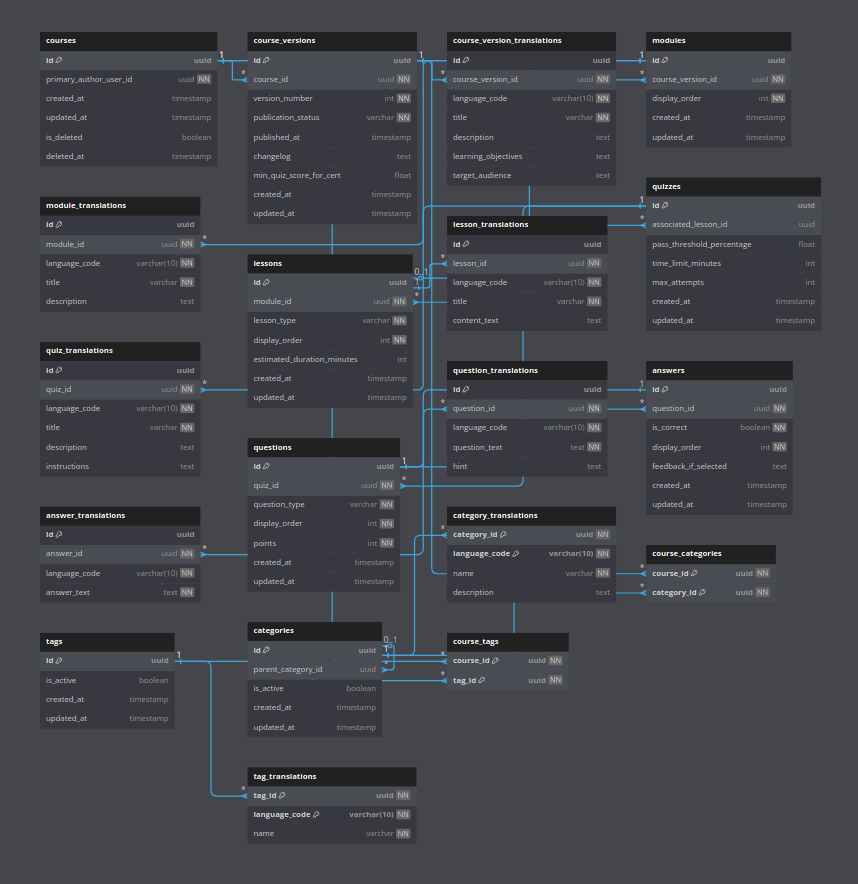
\includegraphics[width=0.8\textwidth,keepaspectratio]{services_db_screanshots/Screenshot 2025-06-06 at 15-07-51 Content_Service.pdf.png}
  \caption{\textbf{Modèle de données du service de contenu} pour la gestion des cours et du matériel pédagogique.}
  \label{fig:content_service}
\end{figure}
\vspace{-10pt}
\small
\paragraph{Points clés du service de Contenu :}
\begin{itemize}[leftmargin=*,noitemsep,topsep=0pt]
  \item \textbf{Structure hiérarchique} des cours, modules et leçons
  \item \textbf{Support multimédia} avec gestion des vidéos, documents et quizz
  \item \textbf{Métadonnées riches} pour faciliter la recherche et la catégorisation
  \item \textbf{Gestion des versions} permettant la mise à jour du contenu sans perte d'historique
  \item \textbf{Support multilingue} pour internationaliser le contenu pédagogique
\end{itemize}
\normalsize
\newpage

\subsubsection{Service de Facturation et d'Abonnement}
\begin{figure}[h!]
  \centering
  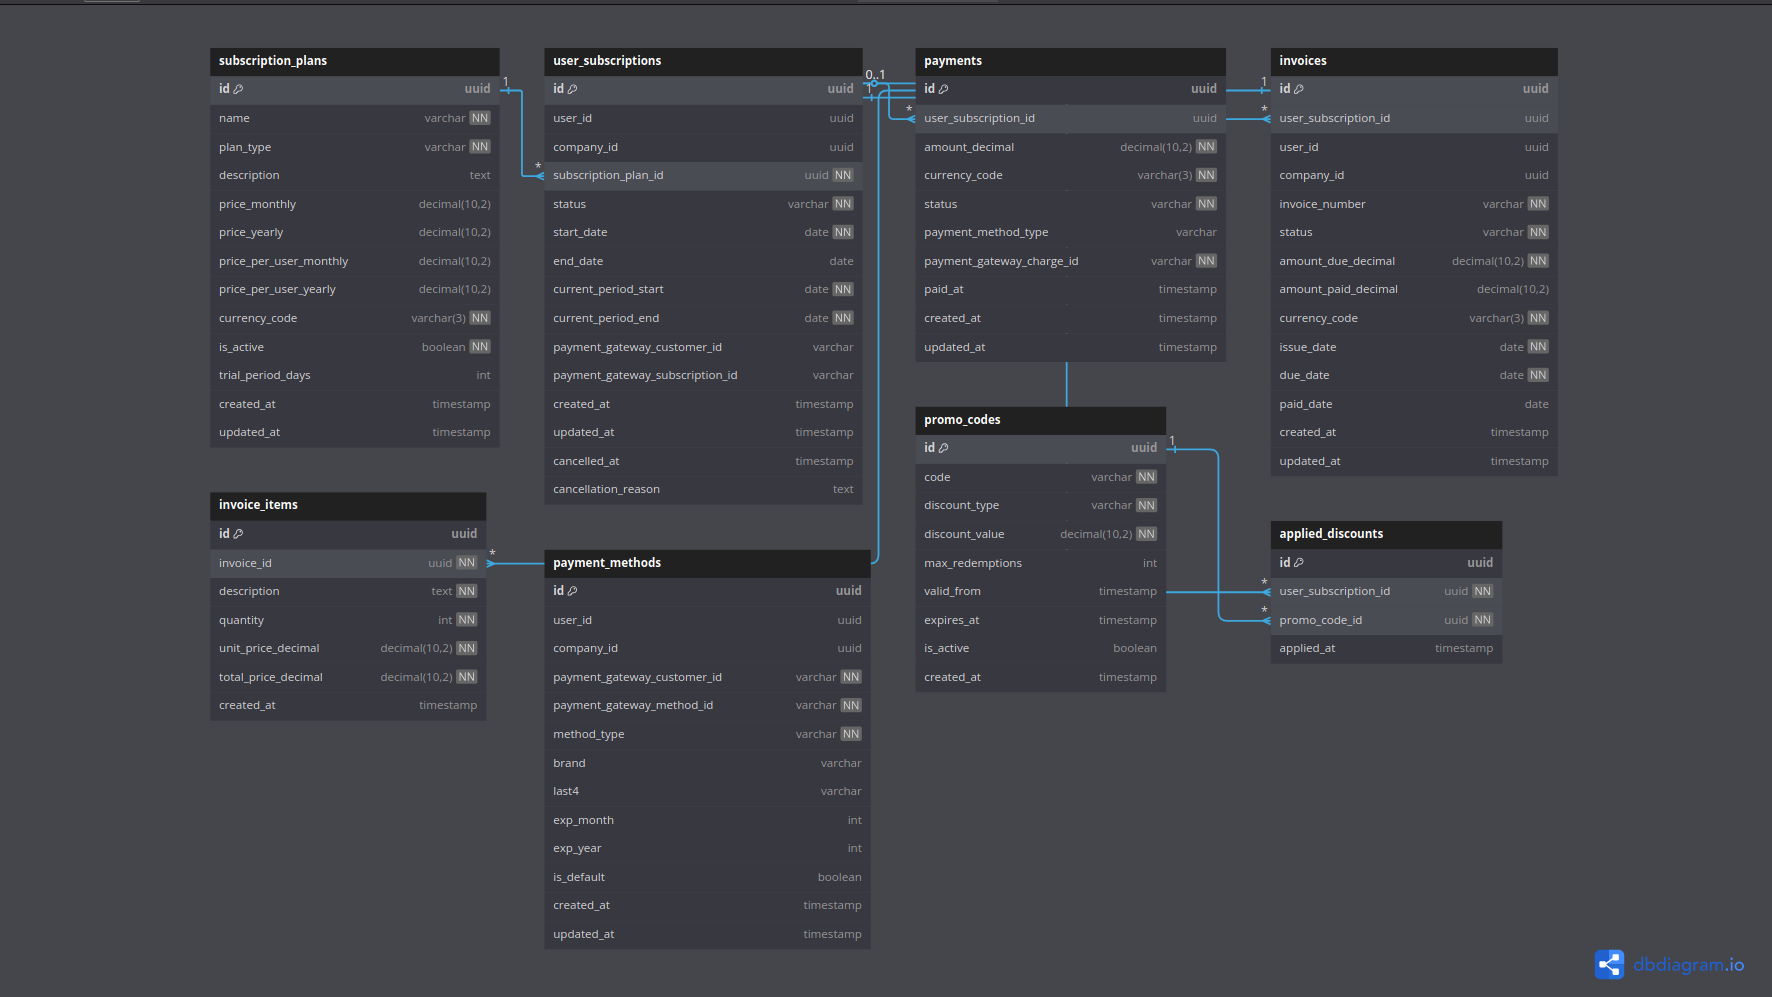
\includegraphics[width=0.8\textwidth,keepaspectratio]{services_db_screanshots/Screenshot 2025-06-06 at 15-05-28 Billing_and_Subscription_Service.pdf.png}
  \caption{\textbf{Modèle de données du service de facturation} pour la gestion des abonnements et des paiements.}
  \label{fig:billing_service}
\end{figure}
\vspace{-10pt}
\small
\paragraph{Points clés du service de Facturation :}
\begin{itemize}[leftmargin=*,noitemsep,topsep=0pt]
  \item \textbf{Gestion des plans d'abonnement} avec différents niveaux de service
  \item \textbf{Suivi des factures et paiements} pour les utilisateurs individuels et entreprises
  \item \textbf{Support des promotions et réductions} temporaires ou permanentes
  \item \textbf{Historique de facturation} complet pour analyses financières
  \item \textbf{Intégration} avec les passerelles de paiement externes
\end{itemize}
\normalsize
\newpage

\subsubsection{Service de Certification}
\begin{figure}[h!]
  \centering
  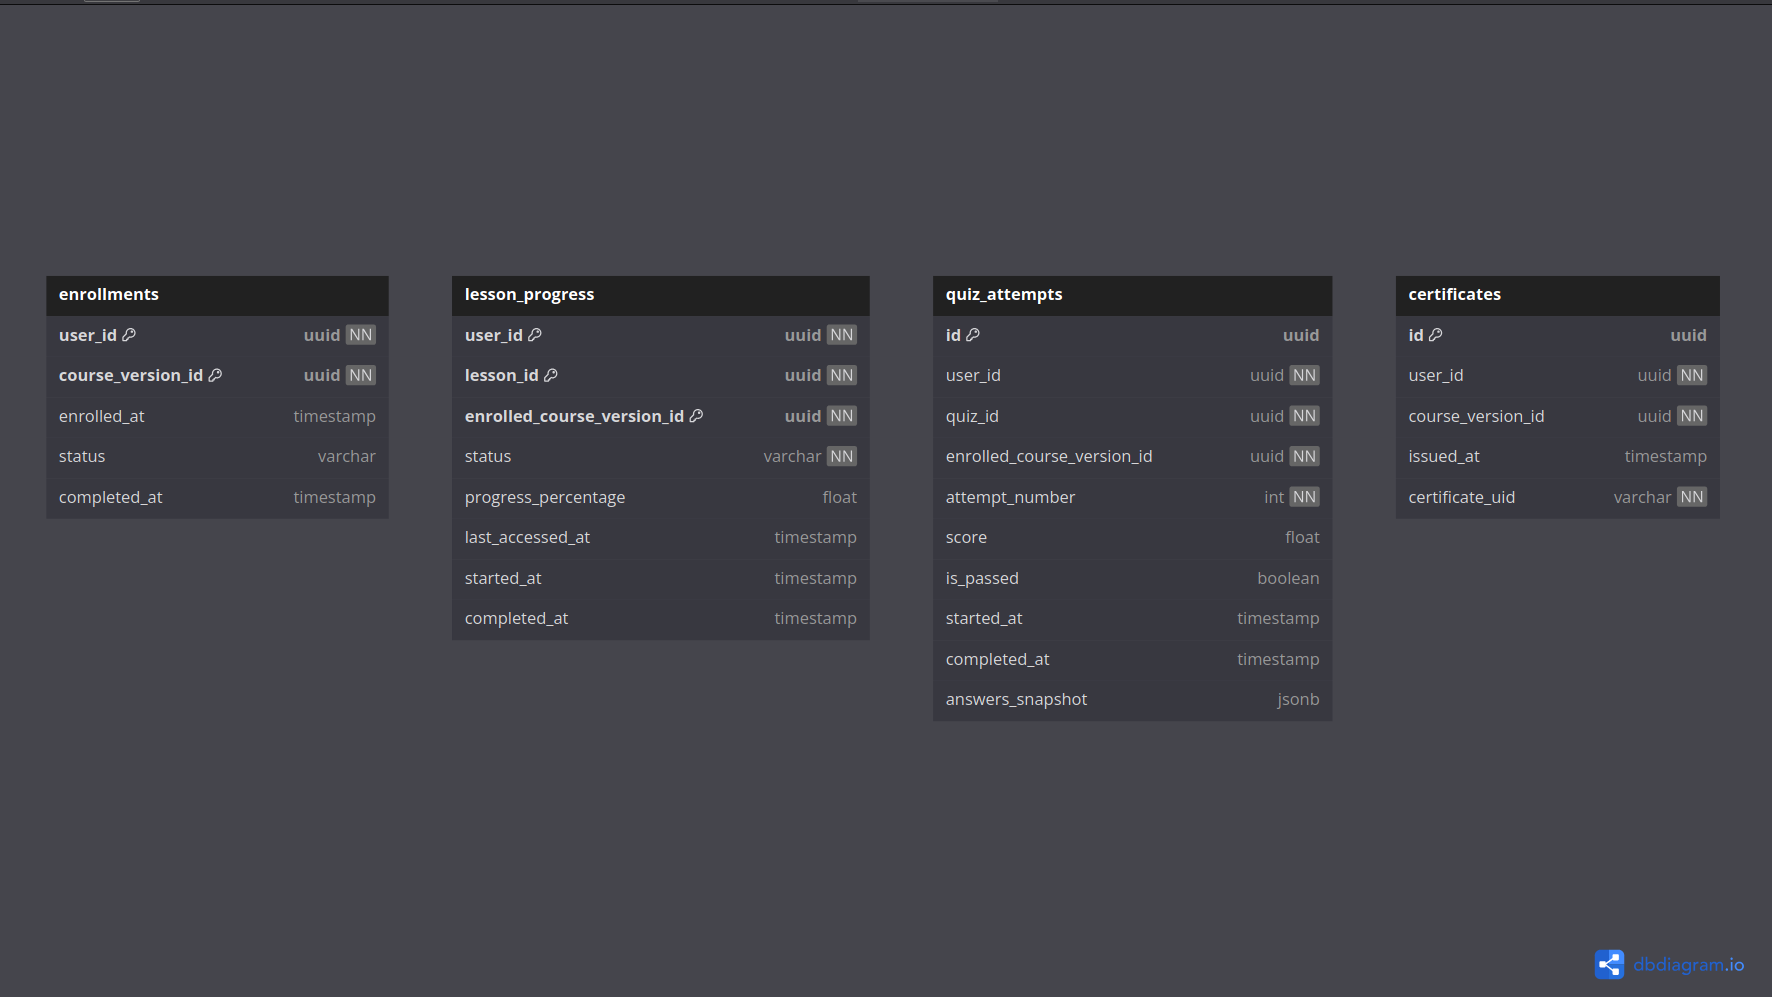
\includegraphics[width=0.8\textwidth,keepaspectratio]{services_db_screanshots/Screenshot 2025-06-06 at 15-05-53 Certification_Service.pdf.png}
  \caption{\textbf{Modèle de données du service de certification} pour la délivrance et la validation des certificats.}
  \label{fig:certification_service}
\end{figure}
\vspace{-10pt}
\small
\paragraph{Points clés du service de Certification :}
\begin{itemize}[leftmargin=*,noitemsep,topsep=0pt]
  \item \textbf{Création de certificats} à l'achèvement des cours et modules
  \item \textbf{Validation et vérification} des compétences acquises
  \item \textbf{Badges et récompenses} pour motiver les apprenants
  \item \textbf{Système de validation externe} permettant aux entreprises de vérifier l'authenticité
  \item \textbf{Historique des certifications} pour chaque utilisateur
\end{itemize}
\normalsize
\newpage

\subsubsection{Service d'Analytique et Reporting}
\begin{figure}[h!]
  \centering
  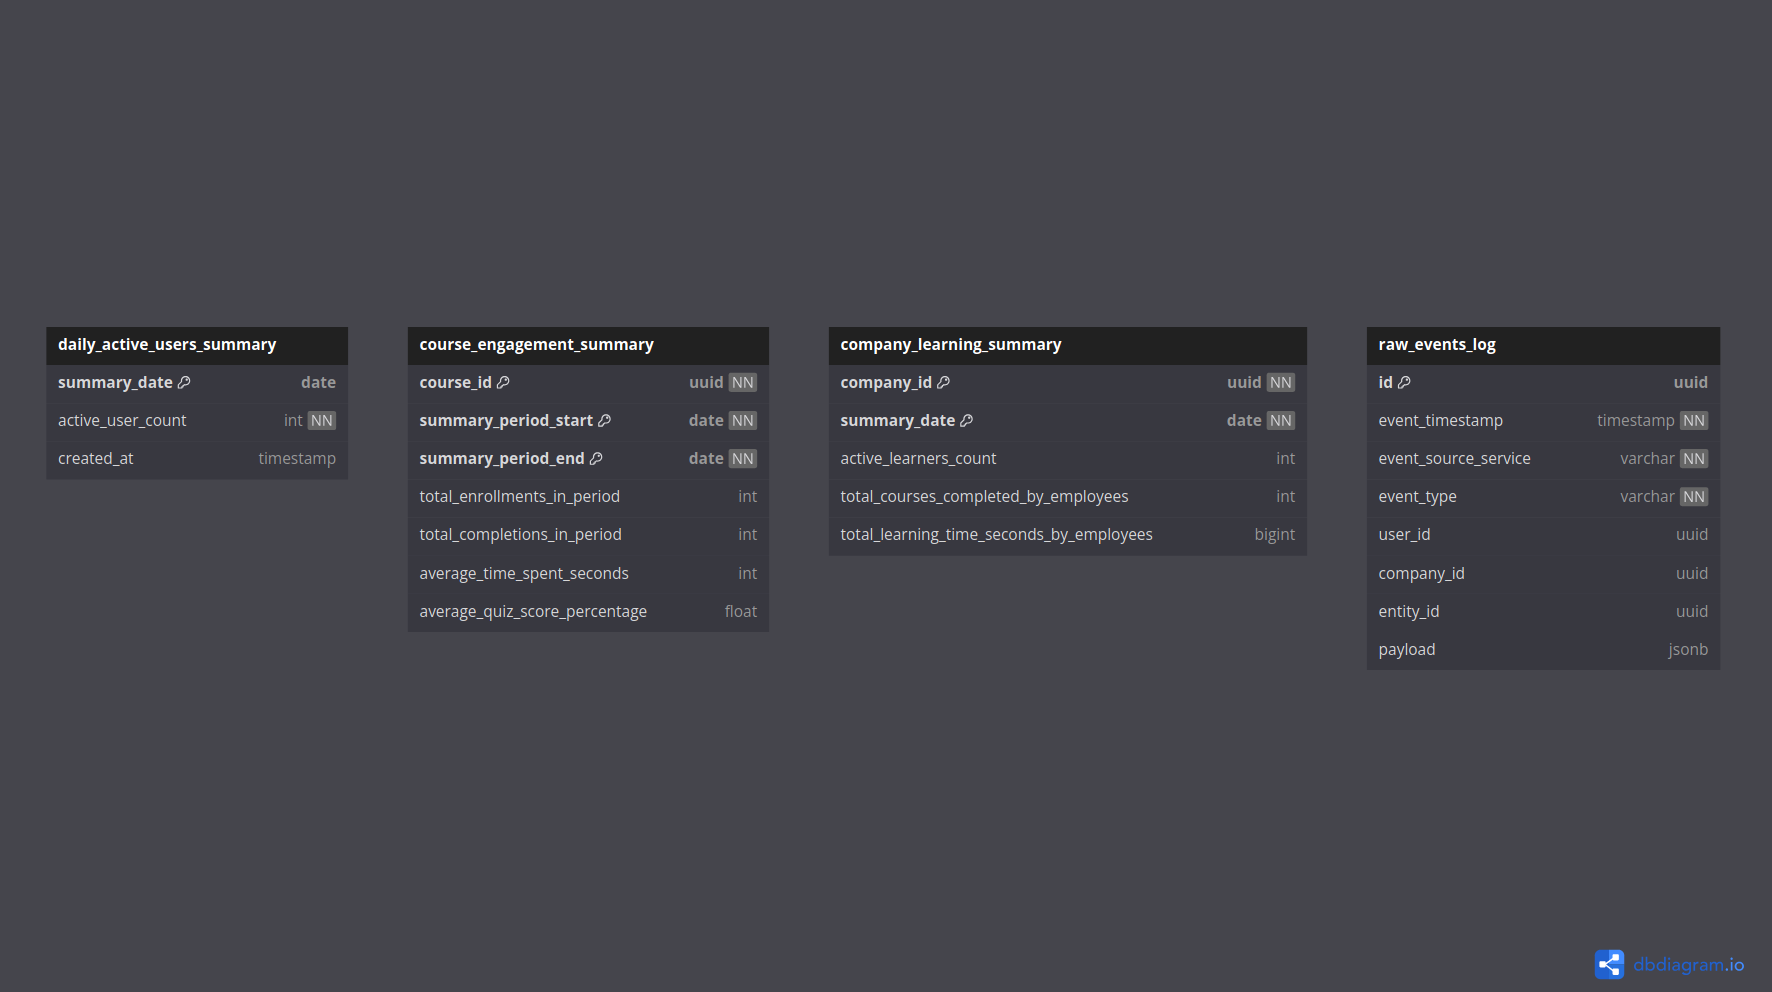
\includegraphics[width=0.8\textwidth,keepaspectratio]{services_db_screanshots/Screenshot 2025-06-06 at 15-04-59 Analytics_and_Reporting_Service.pdf.png}
  \caption{\textbf{Modèle de données du service d'analytique} pour le suivi des performances et la génération de rapports.}
  \label{fig:analytics_service}
\end{figure}
\vspace{-10pt}
\small
\paragraph{Points clés du service d'Analytique :}
\begin{itemize}[leftmargin=*,noitemsep,topsep=0pt]
  \item \textbf{Collecte de données d'utilisation} sur toutes les interactions utilisateurs
  \item \textbf{Métriques de performance} pour les cours et modules
  \item \textbf{Rapports personnalisés} pour les administrateurs et entreprises
  \item \textbf{Tableaux de bord en temps réel} pour le suivi des indicateurs clés
  \item \textbf{Système d'alerte} pour identifier les anomalies ou opportunités
\end{itemize}
\normalsize
\newpage

\subsubsection{Service de Feedback}
\begin{figure}[h!]
  \centering
  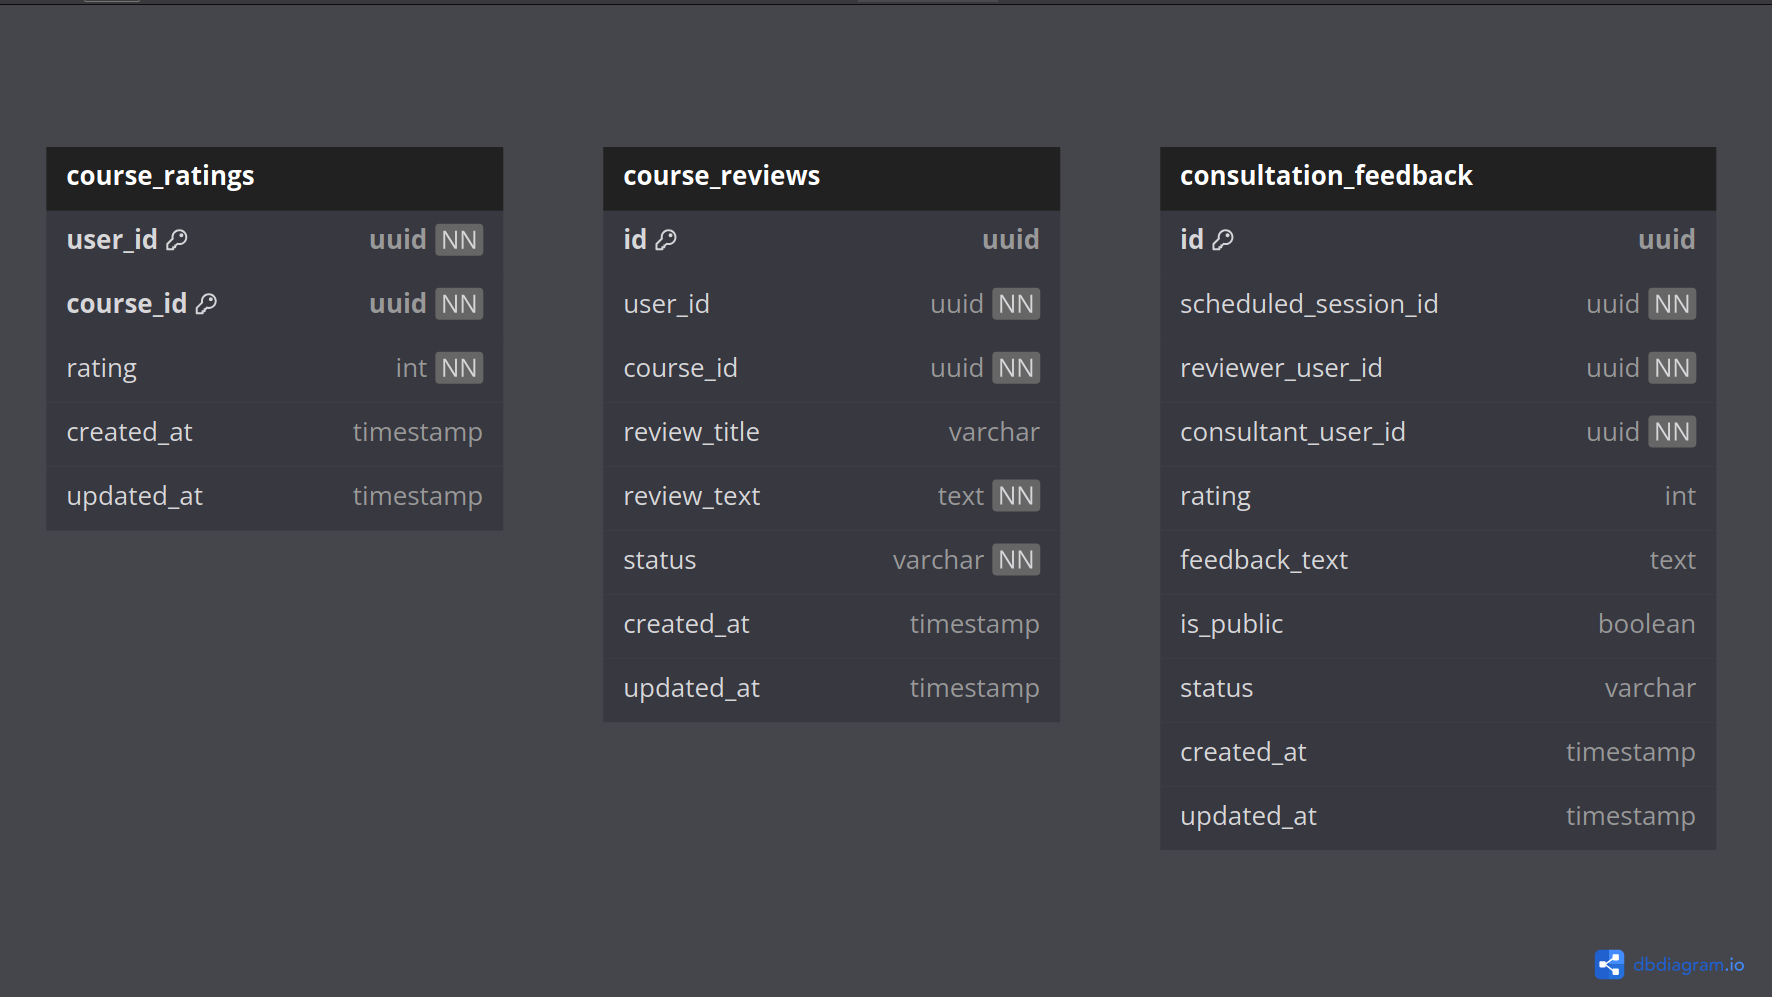
\includegraphics[width=0.8\textwidth,keepaspectratio]{services_db_screanshots/Screenshot 2025-06-06 at 15-08-00 Feedback_Service.pdf.png}
  \caption{\textbf{Modèle de données du service de feedback} pour la collecte et la gestion des retours utilisateurs.}
  \label{fig:feedback_service}
\end{figure}
\vspace{-10pt}
\small
\paragraph{Points clés du service de Feedback :}
\begin{itemize}[leftmargin=*,noitemsep,topsep=0pt]
  \item \textbf{Évaluations et avis} sur les cours et modules
  \item \textbf{Système de notation} permettant une évaluation quantitative
  \item \textbf{Commentaires et suggestions} pour améliorer le contenu
  \item \textbf{Analyse de sentiment} sur les retours textuels
  \item \textbf{Boucle de rétroaction} pour les créateurs de contenu
\end{itemize}
\normalsize
\newpage

\subsubsection{Service de Notification}
\begin{figure}[h!]
  \centering
  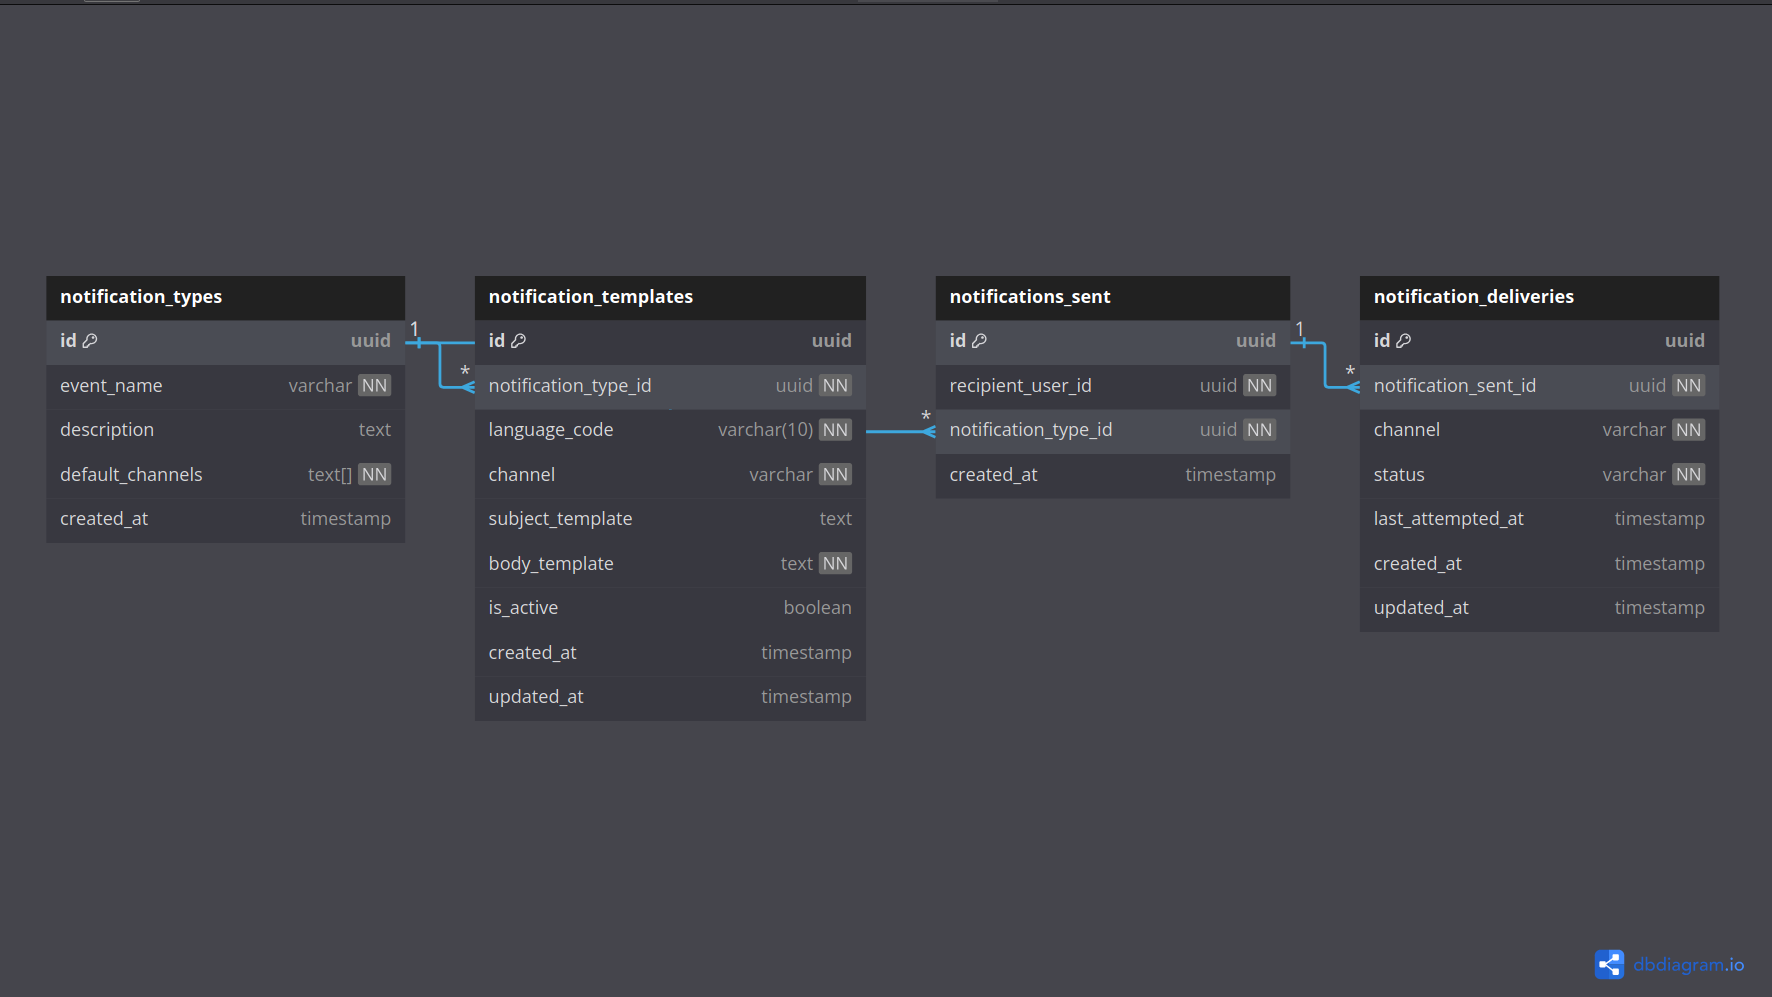
\includegraphics[width=0.8\textwidth,keepaspectratio]{services_db_screanshots/Screenshot 2025-06-06 at 15-08-13 Notification_Service.pdf.png}
  \caption{\textbf{Modèle de données du service de notification} pour l'envoi et la gestion des notifications.}
  \label{fig:notification_service}
\end{figure}
\vspace{-10pt}
\small
\paragraph{Points clés du service de Notification :}
\begin{itemize}[leftmargin=*,noitemsep,topsep=0pt]
  \item \textbf{Notifications temps réel} pour les événements importants
  \item \textbf{Préférences de notification} configurables par utilisateur
  \item \textbf{Support multi-canal} : email, push, in-app, SMS
  \item \textbf{Modèles de messages} personnalisables
  \item \textbf{Planification et automatisation} des campagnes de notification
\end{itemize}
\normalsize
\newpage

\subsubsection{Service de Gestion des Médias}
\begin{figure}[h!]
  \centering
  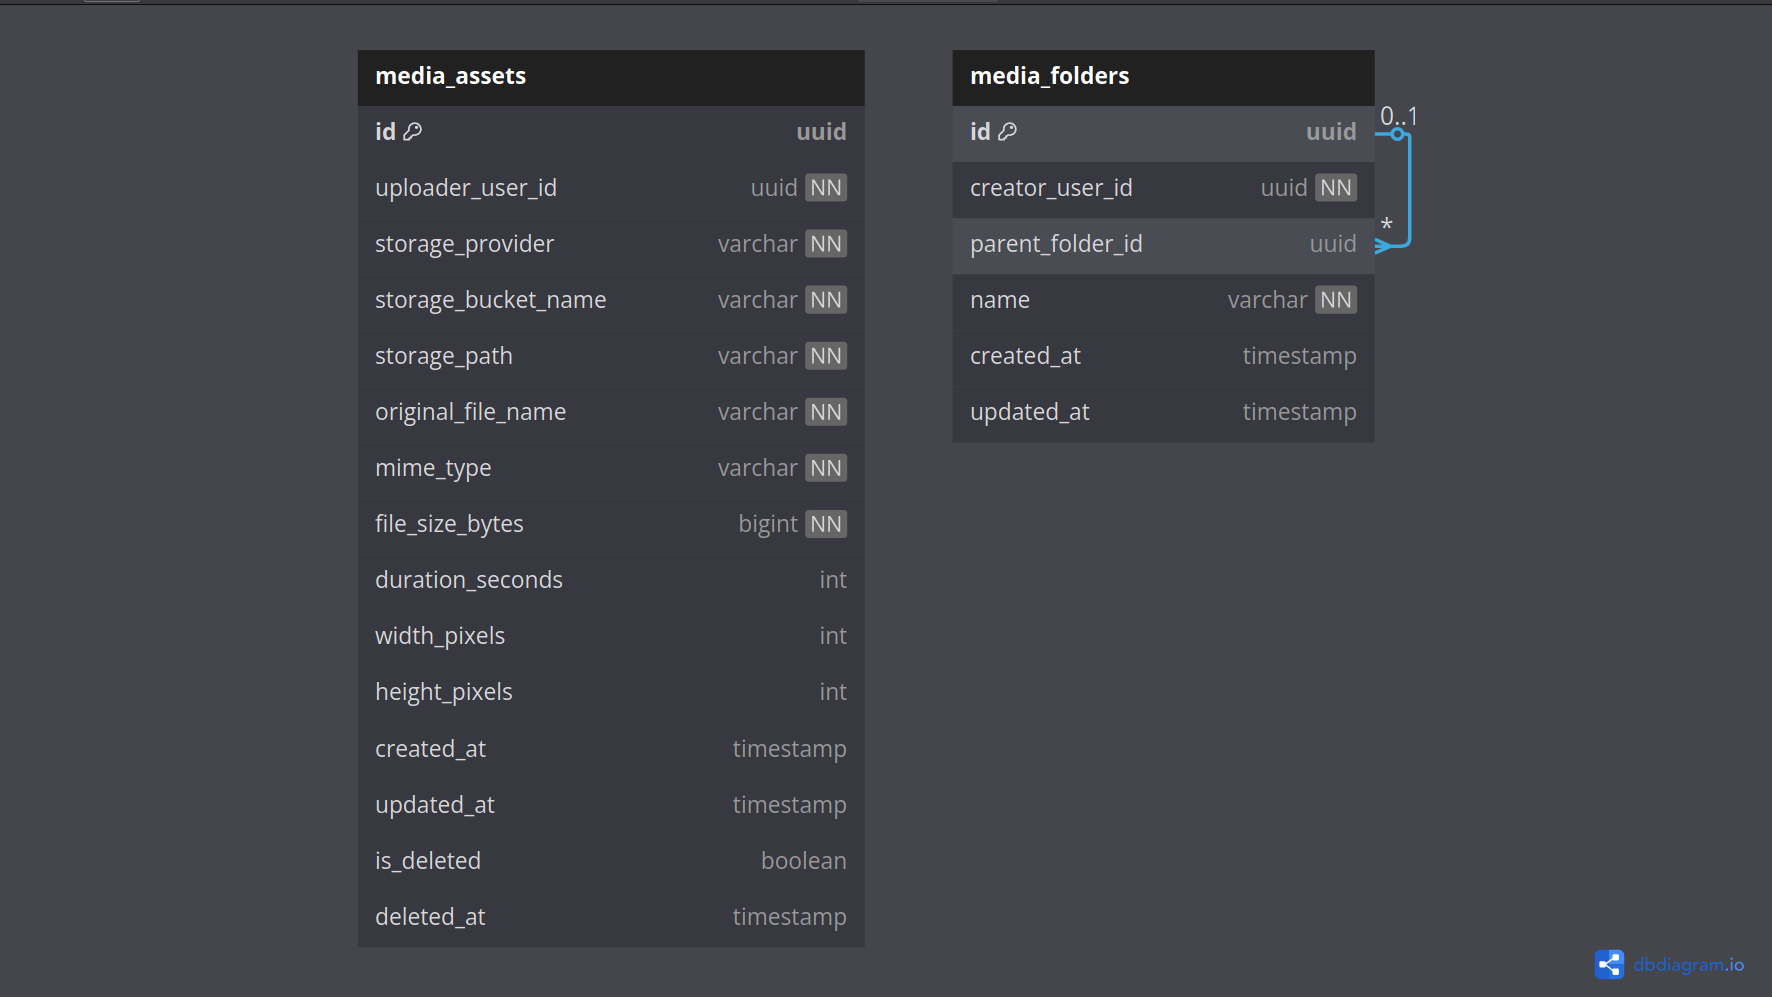
\includegraphics[width=0.8\textwidth,keepaspectratio]{services_db_screanshots/Screenshot 2025-06-06 at 15-08-27 Media_Management_Service.pdf.png}
  \caption{\textbf{Modèle de données du service de gestion des médias} pour le stockage et l'accès aux ressources multimédias.}
  \label{fig:media_service}
\end{figure}
\vspace{-10pt}
\small
\paragraph{Points clés du service de Médias :}
\begin{itemize}[leftmargin=*,noitemsep,topsep=0pt]
  \item \textbf{Gestion centralisée} des ressources audio, vidéo et images
  \item \textbf{Métadonnées enrichies} pour faciliter la recherche et l'organisation
  \item \textbf{Support de multiples formats} et résolutions
  \item \textbf{Optimisation automatique} pour différents appareils
  \item \textbf{Contrôle des droits d'accès} pour les ressources protégées
\end{itemize}
\normalsize
\newpage

\subsubsection{Service de Configuration de la Plateforme}
\begin{figure}[h!]
  \centering
  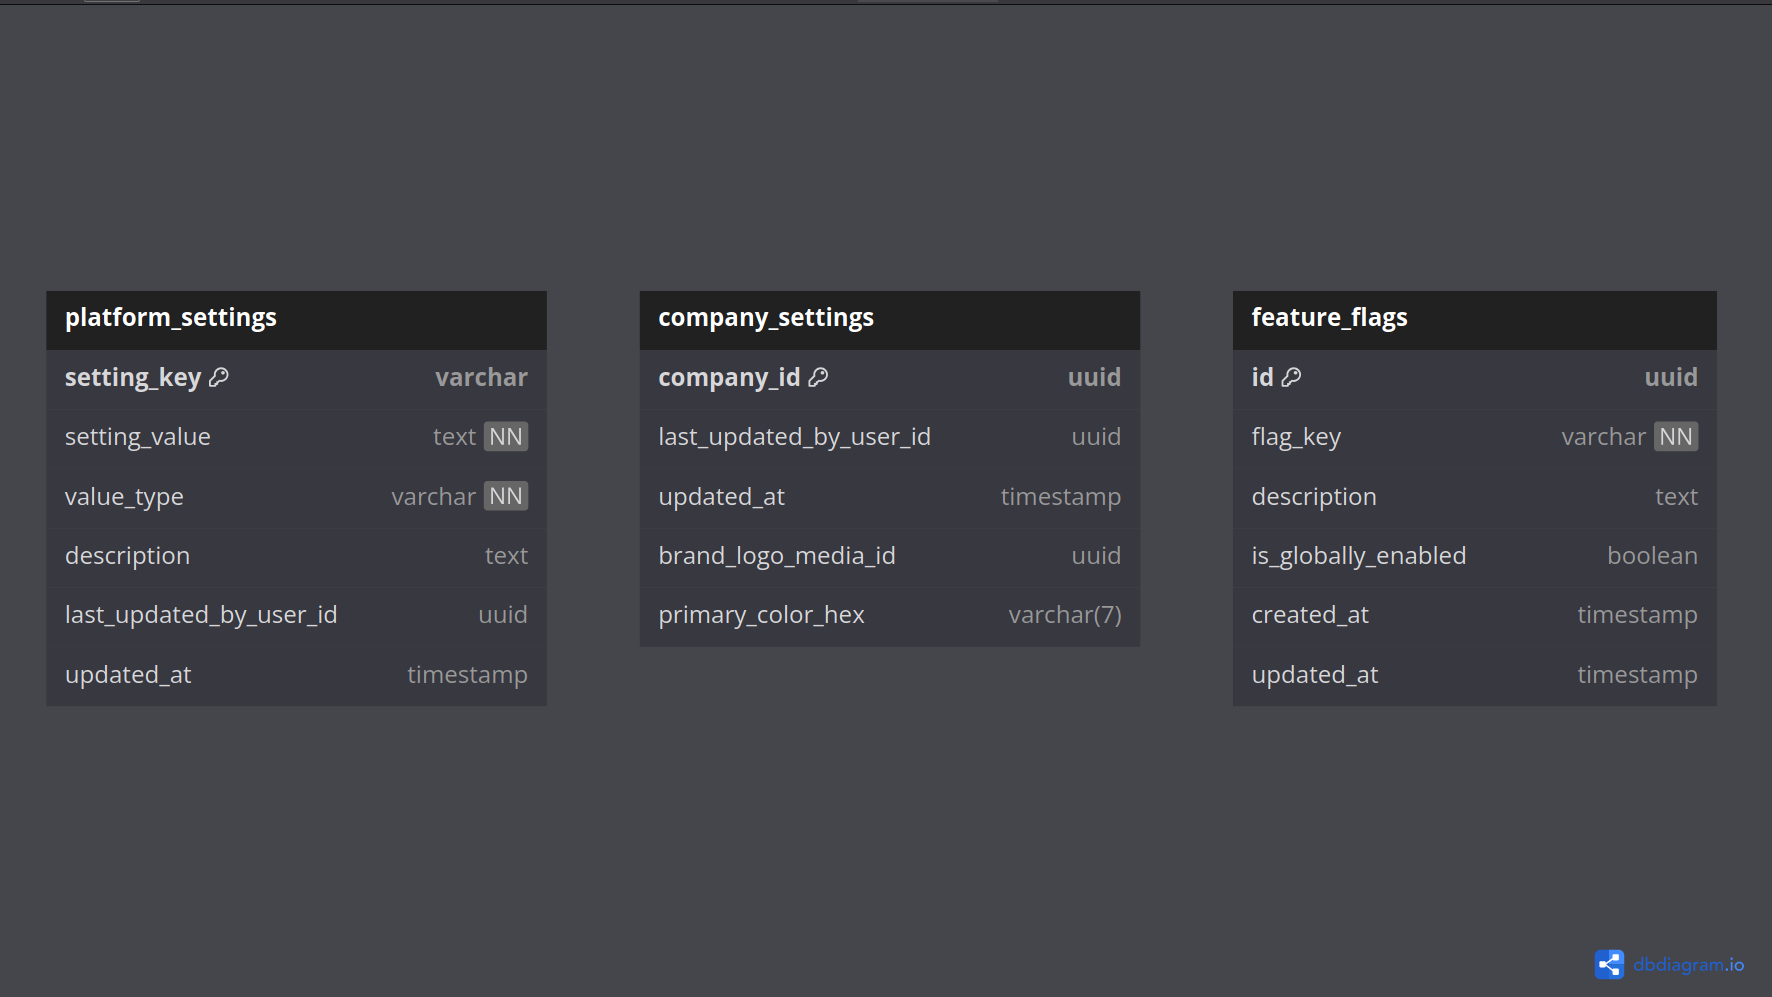
\includegraphics[width=0.8\textwidth,keepaspectratio]{services_db_screanshots/Screenshot 2025-06-06 at 15-08-44 Platform_Configuration_Service.pdf.png}
  \caption{\textbf{Modèle de données du service de configuration} pour la gestion des paramètres globaux de la plateforme.}
  \label{fig:platform_config_service}
\end{figure}
\vspace{-10pt}
\small
\paragraph{Points clés du service de Configuration :}
\begin{itemize}[leftmargin=*,noitemsep,topsep=0pt]
  \item \textbf{Paramètres système} centralisés et accessibles à tous les services
  \item \textbf{Gestion des drapeaux de fonctionnalités} (feature flags)
  \item \textbf{Configuration par environnement} (développement, test, production)
  \item \textbf{Personnalisation de l'interface} selon les besoins spécifiques
  \item \textbf{Paramètres multilingues} pour localisation de la plateforme
\end{itemize}
\normalsize
\newpage

\subsubsection{Service de Recherche}
\begin{figure}[h!]
  \centering
  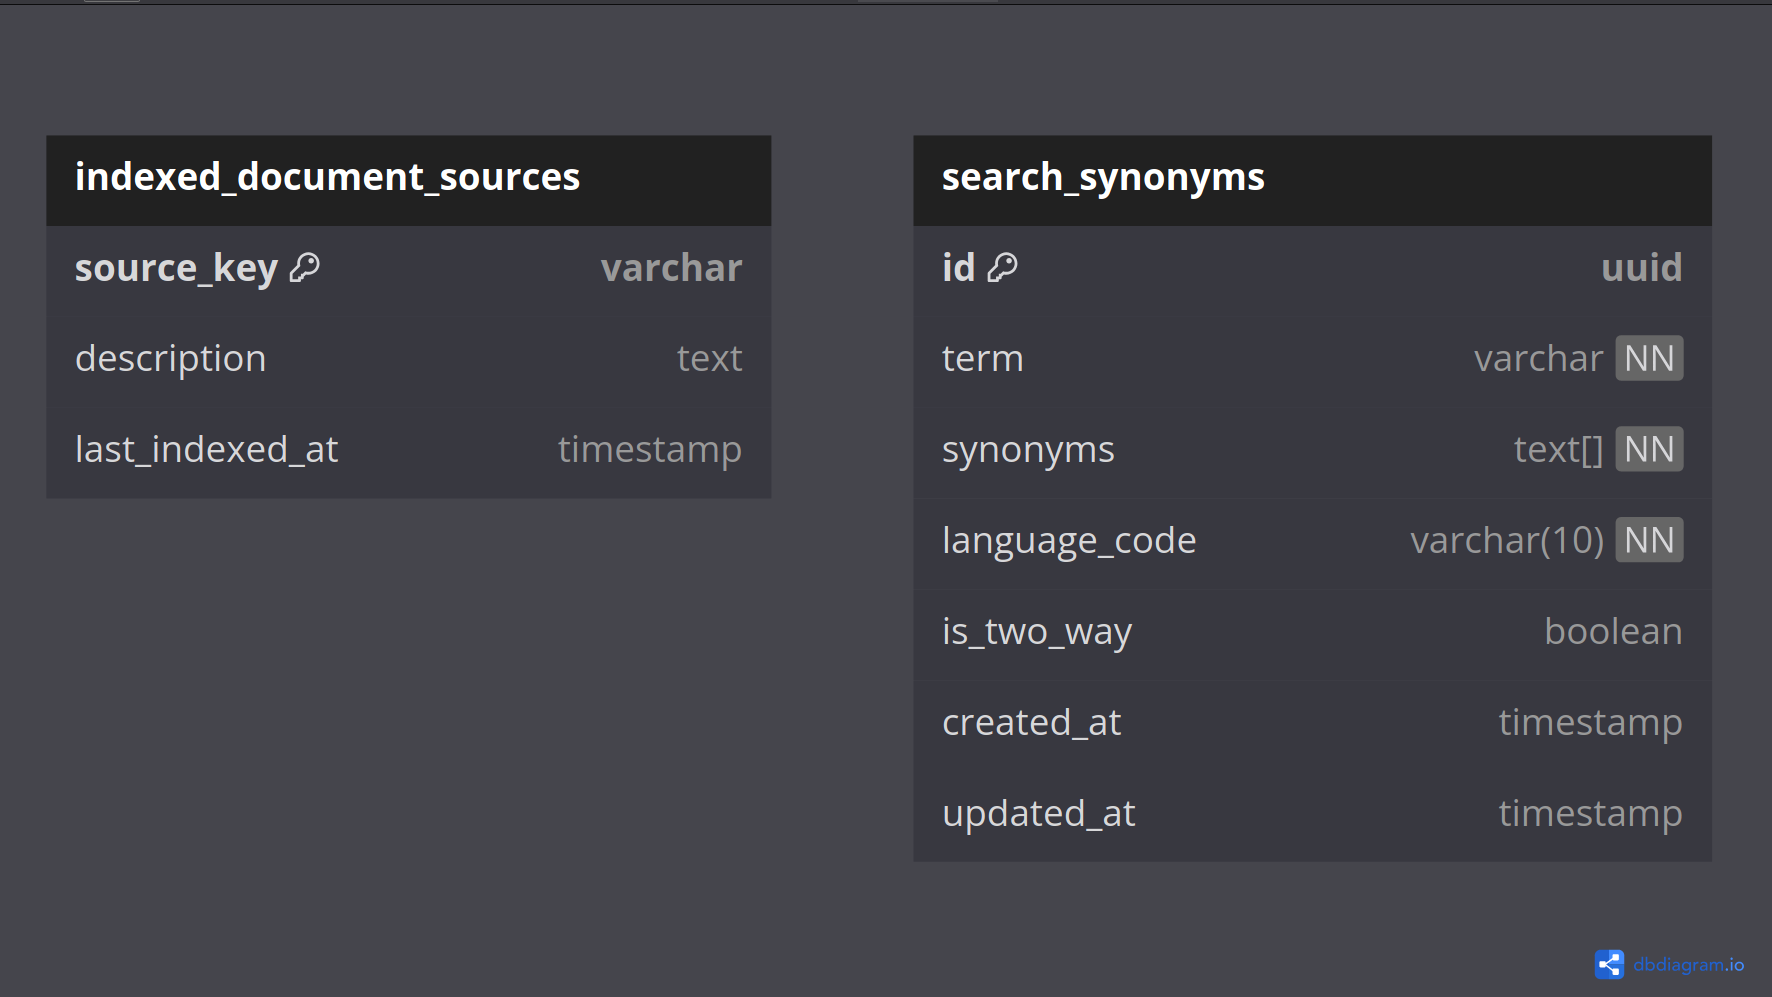
\includegraphics[width=0.8\textwidth,keepaspectratio]{services_db_screanshots/Screenshot 2025-06-06 at 15-08-52 Search_Service.pdf.png}
  \caption{\textbf{Modèle de données du service de recherche} pour l'indexation et la recherche de contenu.}
  \label{fig:search_service}
\end{figure}
\vspace{-10pt}
\small
\paragraph{Points clés du service de Recherche :}
\begin{itemize}[leftmargin=*,noitemsep,topsep=0pt]
  \item \textbf{Indexation intelligente} du contenu des cours et ressources
  \item \textbf{Recherche full-text} avec prise en charge des synonymes
  \item \textbf{Système de tags} pour améliorer la pertinence des résultats
  \item \textbf{Historique des recherches} pour l'analyse des tendances
  \item \textbf{Algorithme de recommandation} basé sur les comportements de recherche
\end{itemize}

\begin{table}[h!]
\centering
\small
\caption{Comparaison des caractéristiques techniques des services}
\label{tab:comparaison_services}
\begin{tabular}{|l|c|c|c|}
\hline
\textbf{Service} & \textbf{Technologie principale} & \textbf{Type de données} & \textbf{Complexité} \\
\hline
IAM & Node.js/Go & Utilisateurs & Élevée \\
Contenu & Python/FastAPI & Éducation & Moyenne \\
Facturation & Python/FastAPI & Financières & Élevée \\
Certification & Python/Go & Validation & Moyenne \\
Analytique & Python & Statistiques & Élevée \\
Feedback & Node.js & Évaluation & Basse \\
Notification & Go & Messaging & Moyenne \\
Médias & Node.js & Binaires & Élevée \\
Configuration & Go & Paramètres & Basse \\
Recherche & Python/Elasticsearch & Index & Élevée \\
\hline
\end{tabular}
\end{table}
\normalsize 